\chapter{Exploring unsupervised domain adaptation techniques} \label{chap:domain-adaptation}

In this chapter we explore unsupervised domain adaptation methods for detecting political bias in Reddit comments, using the cross-domain dataset developed in Chapter \ref{chap:reddit-data}. We consider a direct transfer approach, and an approach using a state-of-the-art domain-adaptive BERT model called AdaptaBERT.

First we introduce some transfer learning notation, which we will use throughout Chapters \ref{chap:domain-adaptation} and \ref{chap:extending-adaptabert}.

\section{Notation}

Let $ A \rightarrow B $ denote some transfer from domain A to domain B, i.e. an $ A \rightarrow B $ model is a transfer learning model from source domain $ A $ to target domain $ B $. This will commonly involve training on some combination of domains A and B, and then making inferences on domain B.

We denote a standard classifier for domain $ B $ as an \textit{in-domain} model for domain B. Even though this is not a transfer learning classifier, we say the source domain and target domain are both B. An in-domain model for domain B provides a theoretical upper-bound for the accuracy of an $ A \rightarrow B $ model \cite{adaptabert}, since any $ A \rightarrow B $ model will most-likely never be able to achieve the same accuracy as a model that has been trained solely on target domain B for inference on B.

\section{Direct transfer} \label{sec:direct-transfer}

\textit{Direct transfer} is the simplest form of domain adaptation. An $ A \rightarrow B $ direct transfer model undergoes training solely on domain $ A $, followed by inference on domain $ B $ and appropriate evaluation metrics being recorded. A diagram of the process is shown in Figure \ref{fig:direct-transfer}.

\begin{figure}[ht]
    \centering
    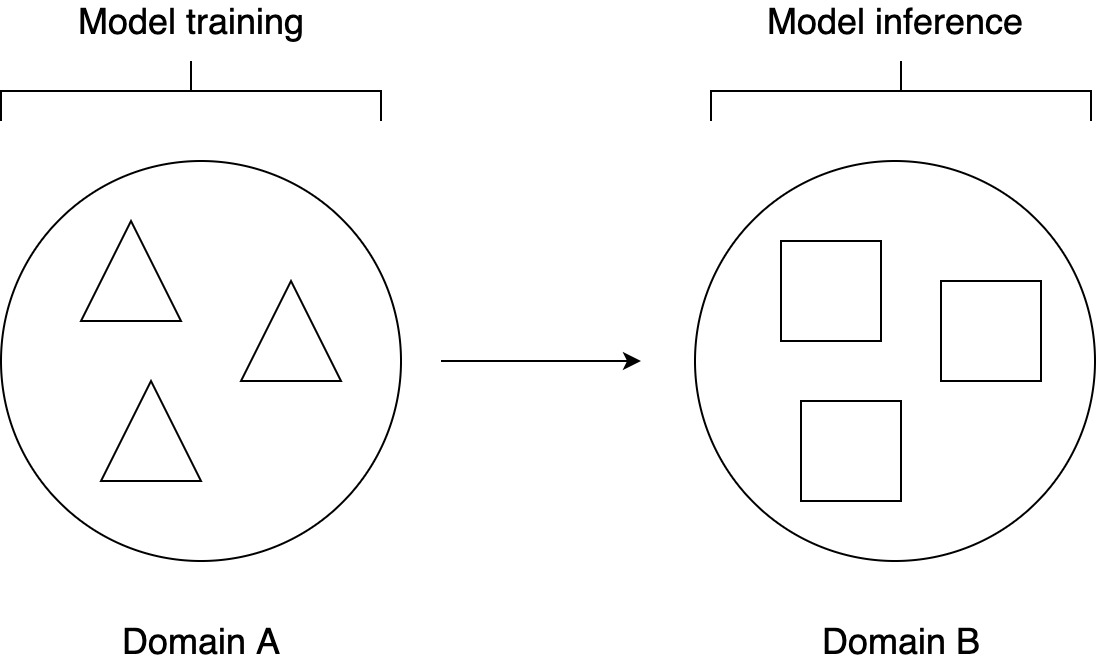
\includegraphics[scale=0.25]{0-img/direct-transfer.png}
    \caption{The direct transfer process (adapted from \cite{ruder})}
    \label{fig:direct-transfer}
\end{figure}

Using our cross-domain Reddit dataset, we will evaluate direct transfer from news articles to comments (denoted as \textit{articles $ \rightarrow $ comments}), and also transfer of comments to news articles (denoted as \textit{comments $ \rightarrow $ articles}). The latter is influenced by the discussion in Section \ref{subsec:readership-bias-social-media} as to whether bias in the news source determines readership bias, or whether bias in the source's audience influences biases in the articles the source produces. Evaluating this transfer will help us see if audience reaction is a good predictor of news article bias. We compare these transfer models against in-domain models for articles and comments.

From Section \ref{sec:domain-similarity}, we identified 3 textual domains in our data. However, news articles can be split up into 2 domains - article headlines and article bodies. We choose to only use article bodies in our investigation, and ignore article headlines - from our results in Section \ref{subsec:nmr-bert-evaluation}, we found that using article body text to detect bias outperforms using any article headline information. From now on when we refer to `articles', we are only considering article body text.

\subsection{Model choice}

In choosing what model to use for our domain adaptation methods, we consider the models explored in Chapter \ref{chap:ensemble-bert}. SVMs and gradient-boosted forests exhibited the best bias-detection performance out of all classifiers, however one major challenge is that these rely on the News-Media-Reliability custom features, which were solely computed for the news sources in that dataset. Recomputing these custom features for every news article and Reddit comment in our cross-domain dataset from Chapter \ref{chap:reddit-data} would be incredibly time-consuming, and so we go with BERT, which performs all feature extraction automatically via examining raw text input. We saw in Section \ref{sec:nmr-bert} that BERT performs slightly worse than the News-Media-Reliability classifiers, however overall its performance is still fairly good.

We use BERT sequence classification models for all of the above. With BERT direct transfer models, pre-training is performed in the same way as for standard BERT - on a large amount of English language text sourced from BookCorpus and Wikipedia. Fine-tuning is performed on the source domain, and then inference is performed on the target domain. See Figure \ref{fig:direct-transfer-in-domain-bert} for a diagram comparing direct transfer and in-domain BERT models. The training objective at each stage is shown in bold, with the domain being trained on underneath.

\begin{figure}
    \centering
    \hspace{-1.5cm}
    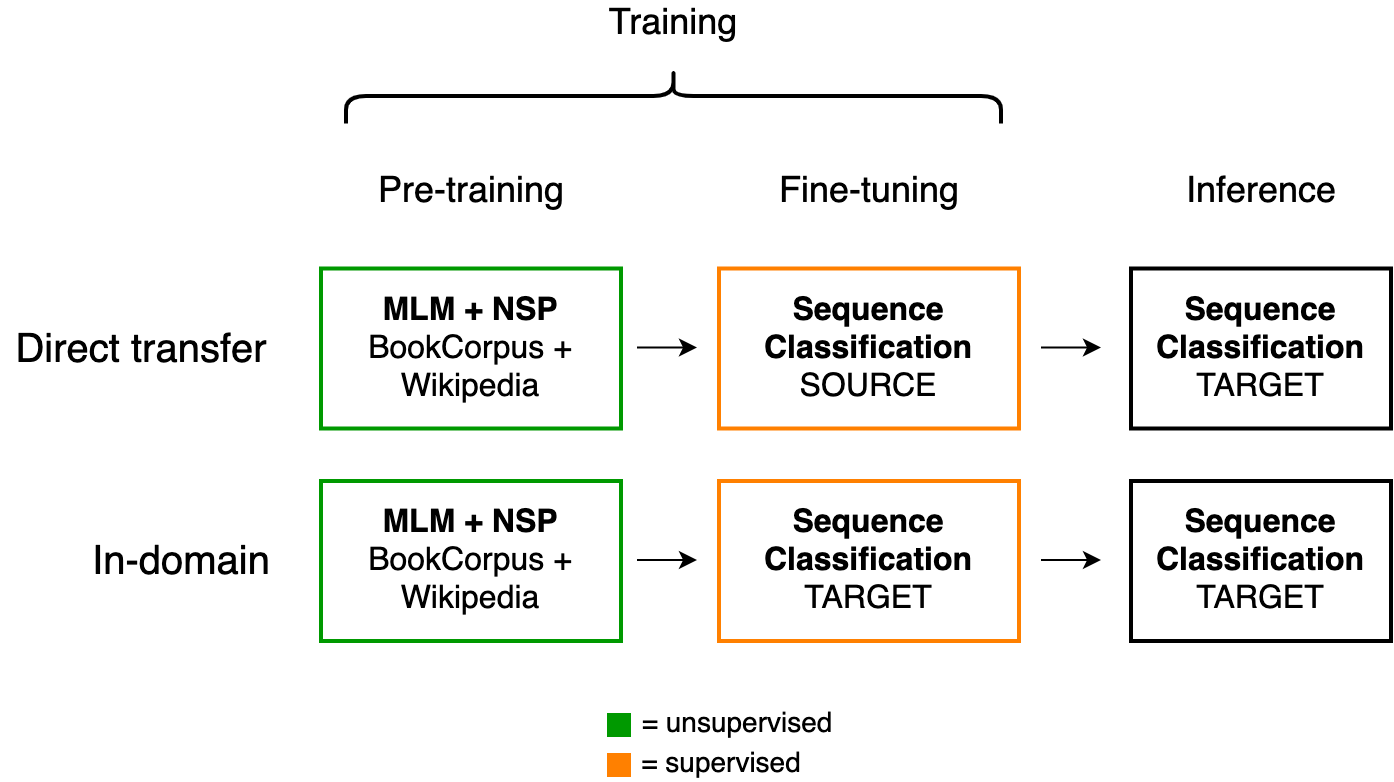
\includegraphics[scale=0.3]{0-img/direct-transfer-in-domain-bert.png}
    \caption{The stages of direct transfer and in-domain BERT approaches}
    \label{fig:direct-transfer-in-domain-bert}
\end{figure}

\subsection{Experimental setup + evaluation}

We use a BERT model for sequence classification based on \texttt{bert-base-uncased}, and perform text preprocessing in a similar fashion to our experiments in Section \ref{sec:nmr-bert}. We also use a train/validation/test split of 70:10:20 to match our Section \ref{sec:nmr-bert} experiments. After tuning hyperparameters we achieve highest accuracies with 5 epochs of training and a batch size of 10.

We evaluate \textit{articles $ \rightarrow $ comments} direct transfer against an in-domain comments model, and \textit{comments $ \rightarrow $ articles} direct transfer against an in-domain articles model. We report macro-averaged F1 score and accuracy for all 4 models. Results are shown in Table \ref{tab:direct-transfer-results}.

Note that the metrics for in-domain models were collected from test-set inference, whereas metrics for the domain adaptation methods were collected from inference over the entire target domain. This is true of all the results we present in Chapters \ref{chap:domain-adaptation} and \ref{chap:extending-adaptabert}.

\begin{table}[ht]
    \centering
    \begin{tabular}{|c|c|c|c|c|}
        \hline
        \textbf{Source Domain} & \textbf{Target Domain} & \textbf{Model Type} & \textbf{Macro-F1} & \textbf{Accuracy} \\
        \hline
        articles & \multirow{2}{4em}{comments} & direct transfer & 54.4 & 51.8 \\
        comments & & in-domain & 67.2 & 67.6 \\
        \hline
        comments & \multirow{2}{3em}{articles} & direct transfer & 69.6 & 69.3 \\
        articles & & in-domain & 76.2 & 76.5 \\
        \hline
    \end{tabular}
    \caption{Evaluation metrics comparing direct transfer to non-transfer baselines}
    \label{tab:direct-transfer-results}
\end{table}

We can see the direct transfer approaches are beaten by the in-domain classifiers in both F1 score and accuracy. The F1 score difference is around 13\% for \textit{articles $ \rightarrow $ comments} transfer, and around 7\% for \textit{comments $ \rightarrow $ articles} transfer. This suggests direct transfer by itself cannot completely substitute for training on the target domain, irrespective of which domain is the target.

The \textit{comments $ \rightarrow $ articles} transfer performs significantly better than \textit{articles $ \rightarrow $ comments}, both in terms of absolute metrics and in terms of how close to the in-domain baseline it is able to achieve. This suggests there is merit to the idea that looking at comments on a particular article are a good predictor for the bias of the article itself. This could be because the number of comments in our dataset is much larger than the number of articles (each article in our dataset has 14 comments on average), so the classifier has access to much more data to train on.

To test this idea, we experiment with reducing the number of comments in the dataset, and re-running the \textit{comments $ \rightarrow $ articles} transfer model. Reducing the number of comments by 50\% results in an accuracy drop of around 5\%, from 69.3\% to 64.5\%, and reducing by 75\% gives a further accuracy drop of 15\%. These are significant drops in accuracy, indicating the sheer number of comments in our dataset contributes to the high accuracy of transfer.

This is an important finding, since in the real world comments are much more abundant in nature than news articles - on articles from mainstream news outlets it is common to find hundreds of comments, both on the site itself and on social media such as Facebook and Reddit. The fact that comment text is a good predictor for news article bias with only a fairly small deterioration in accuracy compared to in-domain methods is something that can be explored further in future work.

\section{AdaptaBERT} \label{sec:adaptabert}

Beyond direct transfer BERT models, we explore a more modern method called AdaptaBERT \cite{adaptabert}, a modified BERT architecture that is geared towards unsupervised domain adaptation.

Standard BERT models are trained for masked language modelling (MLM) and next sentence prediction (NSP) during pre-training, and then are fine-tuned for the task at hand (in our case, sequence classification). In the direct transfer case, this fine-tuning occurs only on the source domain. AdaptaBERT adds an extra fine-tuning step where another round of MLM is performed, but on a combination of the source domain and the target domain. This helps attune BERT's internal contextualised word embeddings to words in the target domain, and yields significantly better performance than direct transfer for the tasks of POS tagging and named entity recognition \cite{adaptabert}, especially on `out-of-vocabulary' (OOV) terms - words seen at inference time in the target domain that were not seen during training.

The new MLM stage is applied to a dataset containing all target domain data available, and an equal amount of source domain data (if the source domain dataset is smaller than the target domain dataset, all source domain data is used). 10 instances of each sample in this dataset are created, each with 15\% of the tokens replaced with [MASK] tokens, following the same procedure as in the original BERT paper \cite{bert}. The model is then trained to predict each masked word.

\begin{figure}[ht]
    \centering
    \hspace{-1.5cm}
    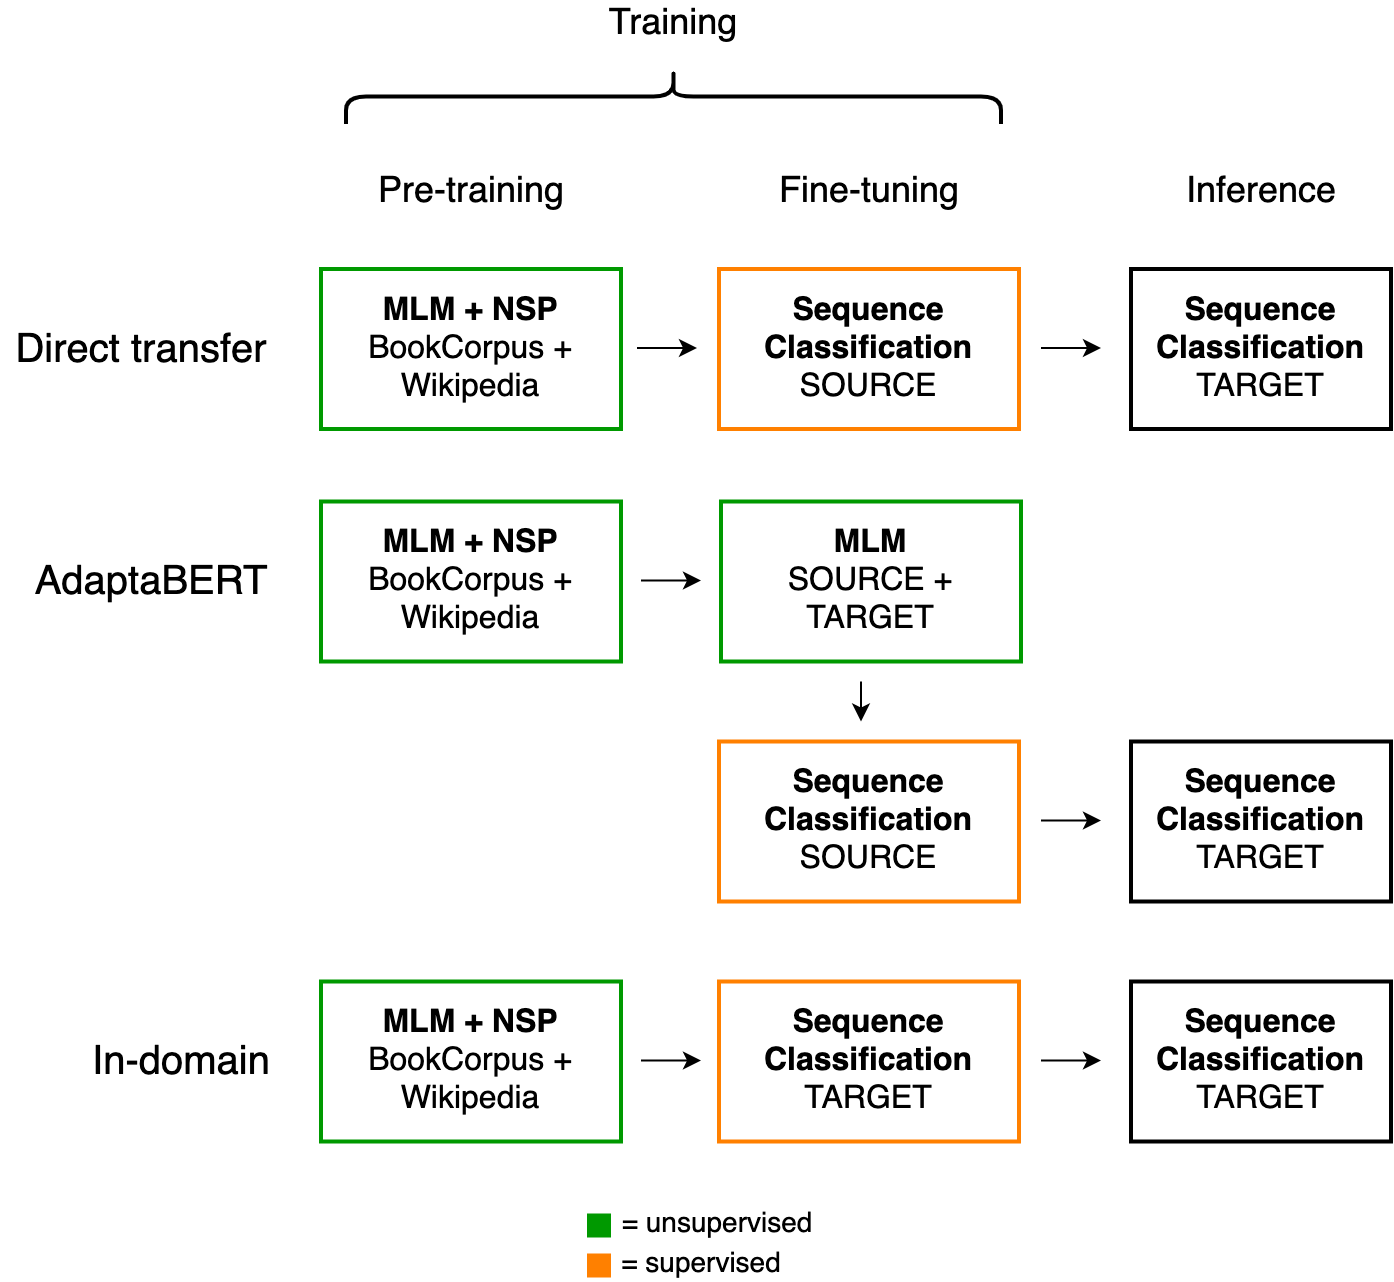
\includegraphics[scale=0.29]{0-img/adaptabert.png}
    \caption{The stages of AdaptaBERT compared to direct transfer and in-domain BERT approaches}
    \label{fig:adaptabert}
\end{figure}

A diagram comparing the AdaptaBERT approach to direct transfer and in-domain approaches is shown in Figure \ref{fig:adaptabert}. We can see AdaptaBERT only adds an extra unsupervised stage, so no extra labelled data is needed in either the source or target domain.

In Section \ref{sec:domain-similarity} we found the Jaccard distance between articles and comments in our dataset was 0.44, indicating good scope for domain adaptation due to a shared vocabulary. However, each of these domains also has a large amount of OOV terms (130,123 for articles and 80,594 for comments). Therefore, our hypothesis is that AdaptaBERT will improve classification performance dramatically over direct transfer.

\subsection{Experimental setup + evaluation} \label{subsec:adaptabert-evaluation}

We modify the code provided by the authors to run AdaptaBERT on our cross-domain Reddit dataset \cite{adaptabert-code}. The new MLM stage is very memory-intensive - we are limited to maximum sequence lengths of 128 tokens instead of the standard 512, as beyond this requires more memory than our hardware can supply. We use a learning rate of $ 5 \cdot 10^{-5} $ and a linear learning rate warm-up period of 10\% of training time as in the AdaptaBERT paper. However we find training with a batch size of 32 for 5 epochs for both the MLM and sequence classification fine-tuning tasks yields better results than the batch size of 64 for 3 epochs as used in the original paper.

Similarly to the previous section, we report results for \textit{articles $ \rightarrow $ comments} transfer as well as \textit{comments $ \rightarrow $ articles} transfer. We compare these against the direct transfer and in-domain baselines for the two domains from Section \ref{sec:direct-transfer}. Results are shown in Table \ref{tab:adaptabert-results} to 3.s.f.

\begin{table}[ht]
    \begin{center}
        \begin{tabular}{|c|c|c|c|c|}
            \hline
            \multicolumn{3}{|c|}{\textbf{Articles $ \rightarrow $ comments transfer}} \\
            \hline
            \textbf{Model Type} & \textbf{Macro-F1} & \textbf{Accuracy} \\
            \hline
            Direct transfer & 54.4 & 51.8  \\
            AdaptaBERT & 50.1 & 55.1 \\
            \hline
            In-domain & 67.2 & 67.6 \\
            \hline
        \end{tabular}
    \end{center} \vspace{10pt}
    \begin{center}
        \begin{tabular}{|c|c|c|}
            \hline
            \multicolumn{3}{|c|}{\textbf{Comments $ \rightarrow $ articles transfer}} \\
            \hline
            \textbf{Model Type} & \textbf{Macro-F1} & \textbf{Accuracy} \\
            \hline
            Direct transfer & 69.6 & 69.3  \\
            AdaptaBERT & 69.7 & 69.8 \\
            \hline
            In-domain & 76.2 & 76.5  \\
            \hline
        \end{tabular}
    \end{center}
    \caption{Evaluation metrics comparing AdaptaBERT to direct transfer and in-domain baselines}
    \label{tab:adaptabert-results}
\end{table}

We can see AdaptaBERT gives slightly mixed results for \textit{articles $ \rightarrow $ comments} transfer, outperforming in terms of accuracy by around 4\%, however letting F1 suffer by a similar amount. In the \textit{comments $ \rightarrow $ articles} case AdaptaBERT outperforms direct transfer slightly, but not in a statistically significant way. We can see in both directions, both direct transfer and AdaptaBERT fall short of the in-domain upper bound, however again the difference is much less in the \textit{comments $ \rightarrow $ articles} case.

Han \& Eisenstein implement AdaptaBERT for a named entity recognition task on social media, examining transfer from news text to Twitter content \cite{adaptabert}. They find AdaptaBERT gives a 1\% improvement in F1 score over direct transfer (58.9\% vs 57.7\%), and this extends to 3\% when AdaptaBERT undergoes MLM on 1 million extra tweets. Further work could be to collect larger amounts of Reddit data and experiment running AdaptaBERT again - our Reddit dataset is fairly small, with just over 10,000 comments.

\subsection{Finding the optimal proportion of source domain examples for MLM} \label{subsec:src-proportion-adaptabert}

In standard AdaptaBERT, an equal amount of source domain and target domain examples are used for the novel MLM stage. We experiment with varying the amount of source domain content used relative to target domain content to see if we can improve classifier accuracy.

We evaluate AdaptaBERT for both \textit{articles $ \rightarrow $ comments} transfer and \textit{comments $ \rightarrow $ articles} transfer, with source proportion values of 0, 1/3, 2/3 and 1 (where `source proportion' = number of source domain examples as a proportion of target domain examples). For each experiment we always use all target domain data available. Results are shown in Figure \ref{fig:src-proportion}.

\begin{figure}[ht]
    \centering
    \begin{subfigure}{\textwidth}
        \centering
        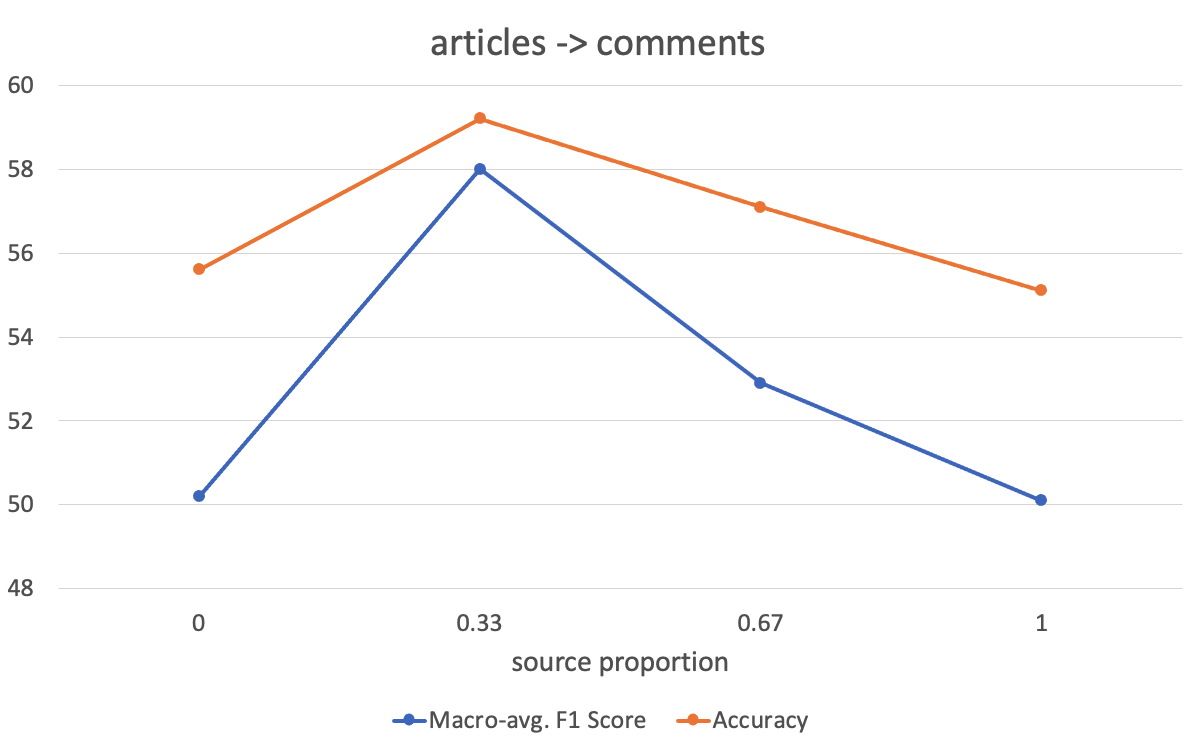
\includegraphics[scale=0.3]{0-img/src-proportion-articles-comments.png}
    \end{subfigure}
    \begin{subfigure}{\textwidth}
        \centering
        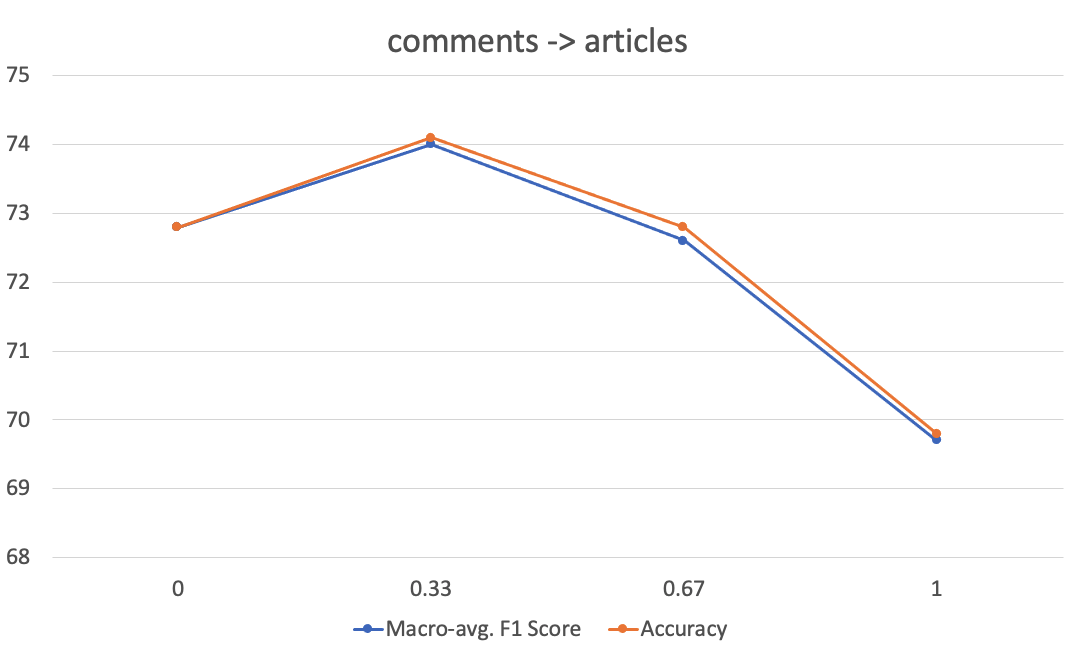
\includegraphics[scale=0.3]{0-img/src-proportion-comments-articles.png}
    \end{subfigure}
    \caption{Performance of AdaptaBERT when varying proportion of source domain examples compared to target domain examples used in the MLM stage}
    \label{fig:src-proportion}
\end{figure}

We can see for both directions of transfer, using 1/3 of the number of target domain examples for the source domain provides the both the best F1 score and accuracy. Compared to using an equal amount of source and target domain examples (a source proportion of 1), this boosts F1 scores by around 8\% to 58.0\% for \textit{articles $ \rightarrow $ comments} transfer and by around 4\% to 74.0\% for \textit{comments $ \rightarrow $ articles} transfer. This is a significant improvement over the results in Table \ref{tab:adaptabert-results}. Note that in the \textit{comments $ \rightarrow $ articles} case, this puts us only around 2\% short of the in-domain baseline.

There is a general trend of increasing deterioration in classification performance the more source domain material is added to the MLM stage - this shows us classification performance is highest when the amount of source domain material used is fairly low compared to target domain material. This makes sense, since after a point adding more source domain material could attune BERT's internal contextualised embeddings too much towards source domain material, and could cause it to start `forgetting' some target domain context. This is linked to a wider problem in neural-network-based models called `catastrophic forgetting' \cite{catastrophic-forgetting}. 